% \begin{frame}{Summary of study}
    
% \end{frame}

\begin{frame}{Publication: Journal articles}
%\resizebox{\textwidth}{!}{%
\begin{tabular}{p{15mm}p{80mm}}
    \tiny{\color{blue}{RPTEL 2020}} & {\small \underline{Sadita,  L.},  Hirashima,  T.,  Hayashi,  Y.,  Furtado,  P.  G.,  Junus,  K.,  and Santoso,  H.  B.  (2020).   The  Effect  of  Differences  in  Group  Composition on Knowledge Transfer, Group Achievement and Learners' Affective Responses During Reciprocal Concept Mapping With The Kit-Build Approach. \textit{Research and Practice in Technology Enhanced Learning}, 15(13).  \href{https://doi.org/10.1186/s41039-020-00133-9}{10.1186/s41039-020-00133-9.}}\\
    \tiny{\color{blue}{IEICE 2020}} & {\small\underline{Sadita, L.}, Furtado, P. G. F., Hirashima, T., and Hayashi, Y. (in press). Analysis of The Similarity of Individual Knowledge and The Comprehension of Partner’s Representation during Collaborative Concept Mapping with Reciprocal Kit Build Approach. \textit{IEICE  TRANSACTIONS  on Information and Systems}, E103-D(7)}. 
\end{tabular}
%}
\end{frame}

\begin{frame}[allowframebreaks]{Publication: International conference papers}
\begin{tabular}{p{15mm}p{80mm}}
    \tiny{\color{blue}{ICCE 2018}} & {\small\underline{Sadita, L.}, Hirashima, T., Hayashi, Y., Wunnasri, W., Pailai, J., Junus, K.,and Santoso, H. B. (2018). Preliminary Study on the Use of Reciprocal Kit Build for Collaborative Learning.  In \textit{The  26th  International  Conference on Computers in Education (ICCE 2018)}, pages 133–142.}\\
    
    \tiny{\color{blue}{ICCE 2019}} & {\small \underline{Sadita,  L.},  Hirashima,  T.,  Hayashi,  Y.,  Furtado,  P.  G.,  Junus,  K.,  and Santoso, H. B. (2019c).  Reciprocal Kit Build Approach for Peer-to-peer Communication:  Relationship between Similarities on Knowledge, Transfer  of  Knowledge,  and  Affective  Responses. In \textit{The  27th International Conference  on  Computers  in  Education  (ICCE  2019)},  volume  1,  pages 101–110.}\\
\end{tabular}

\begin{tabular}{p{15mm}p{80mm}}
    \tiny{\color{blue}{ICCE-DSC 2019}} & {\small \underline{Sadita, L.}, Hirashima, T., and Hayashi, Y. (2019).  Reciprocal Kit Build Concept Map:  An Activity Designed to Encourage Learning at Boundary in Collaborative Situation.  In \textit{The 27th International Conference on Computers in Education (ICCE 2019)}, volume 2, pages 779–782.}
\end{tabular}
\end{frame}

\begin{frame}{Publication: Local conference papers}
\begin{tabular}{p{15mm}p{80mm}}
    \tiny{\color{blue}{ALST 2019}} &\underline{Sadita, L.}, Hirashima, T., Hayashi, Y., et al. (2019b). Reciprocal Kit Build:Boundary Crossing with Concept Map for Collaborative Knowledge Construction. 先進的学習科学と工学研究会, 86:50–55.
\end{tabular}
\end{frame}

\begin{frame}{Thesis structure}
    \begin{figure}[tb]
        \begin{center}
            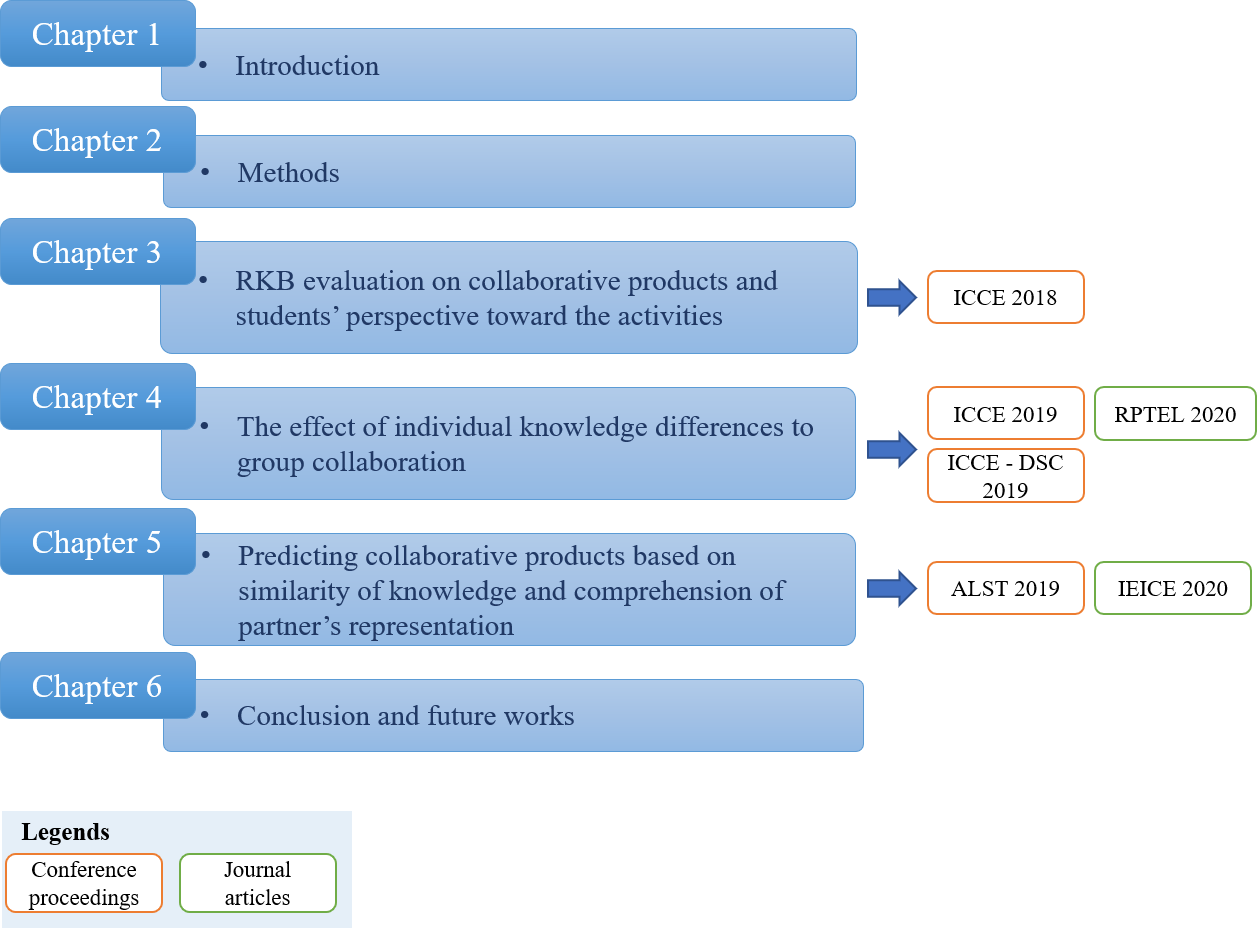
\includegraphics[width=95mm]{images/thesis_structures.pdf} 
        \end{center}
        \caption{Thesis structure and relevant publications}
        \label{thesis_struct}
    \end{figure}
\end{frame}